\section{Ejercicio 6}
\subsection{Introducci\'on}
\noindent
En esta sección se implementará un Latch SR y un Flip Flop D mediante compuertas lógicas en una placa PCB, para luego encontrar conclusiones relevantes sobre las mismas y compararlas con los valores de las compuertas comerciales.
%
\subsection{Latch SR}
\subsubsection{Funcionamiento}
\noindent
Un Latch SR es un circuito encargado de almacenar un valor permitiendo borrar al mismo, es decir actúa como una memoria de 1 bit que permite almacenar o borrar su valor según el valor de sus entradas, para esto presenta una entrada denominada usualmente como Set que se encarga de fijar el valor que se querrá almacenar (cero o uno) y una entrada Reset que se encarga de borrar el valor almacenado haciendo que el mismo valga cero para cualquier valor de set.
%
\subsubsection{Circuito implementado}
\noindent
De esta manera el circuito típico correspondiente al Latch SR se muestra en la figura \ref{ej6_latch_sr} y la tabla de verdad del mismo se puede apreciar en la tabla \ref{ej6_tabla_latch_sr}. \\
%
La entrada S corresponde a la entrada Set y la entrada R refiere a la entrada Reset.
%
%
%
\begin{figure}[H]
    \centering
        \centering
        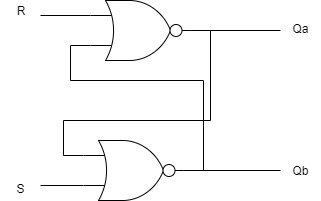
\includegraphics[width=0.5\textwidth]{figs/Ej6/latchsr.jpg} % first figure itself
         \caption{Circuito correspondiente a un Latch SR}
         \label{ej6_latch_sr}
\end{figure}
%
\begin{table}[H]
\caption{Tabla de verdad correspondiente al Latch SR (donde $Qa_{-1}$ refiere al valor que se almacena en el latch.}
\label{ej6_tabla_latch_sr}
\centering
\begin{tabular}{|l|l||l|l|}
\hline
S & R & Qa & Qb \\ \hline \hline
0   & 0     & $Qa_{-1}$     & $Qb_{-1}$     \\ \hline
0   & 1     & 0     & 1   \\ \hline
1   & 0    & 1     & 0   \\ \hline
1   & 1    & 0     & 0   \\ \hline 
\end{tabular}
\end{table}
%
\noindent
De esta forma se trabajó con compuertas NOR para la creación del Latch, para eso se consideró interesante trabajar con compuertas lógicas CD4001B, ya que las mismas son más lentas que las compuertas 74HC02 y hay mayor disponibilidad de ellas en el pañol de la facultad.
%
\subsubsection{Mediciones y Conclusiones.}
%
\noindent
Así se midió el cambio en la salida cuando Reset esta en cero y Set cambia de 0 a 1, de esta forma, en las figuras \ref{ej6_latch_imagen1} y \ref{ej6_latch_imagen2} presentadas a continuación se pueden ver el tiempo de rise y el tiempo de propagación para estas compuertas en estas condiciones. Cabe destacar que la medición de estos valores se realizó con puntas x10 debido a que la medición con puntas x1 se veía muy alterada por el instrumento de medición.
\noindent
\begin{figure}[H]
    \centering
        \centering
        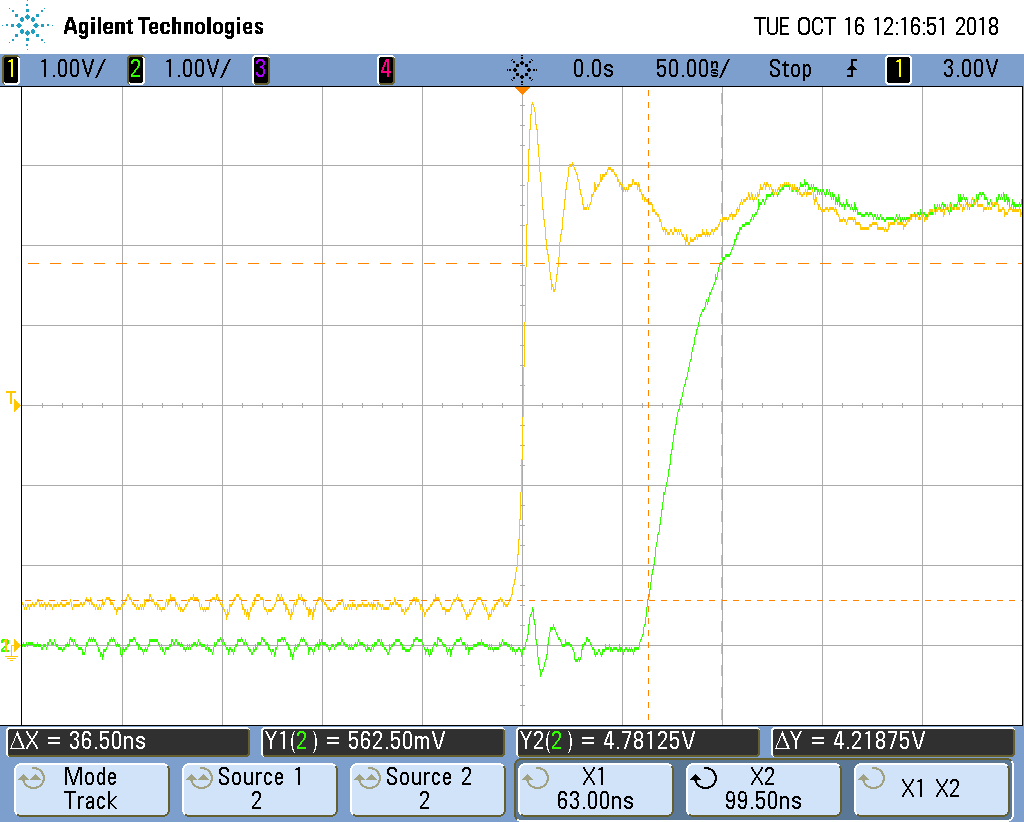
\includegraphics[width=0.6\textwidth]{figs/Ej6/sr_trise.png} % first figure itself
         \caption{Medición correspondiente al tiempo de rise de la compuerta.}
         \label{ej6_latch_imagen1}
\end{figure}
%
%
\begin{figure}[H]
    \centering
        \centering
        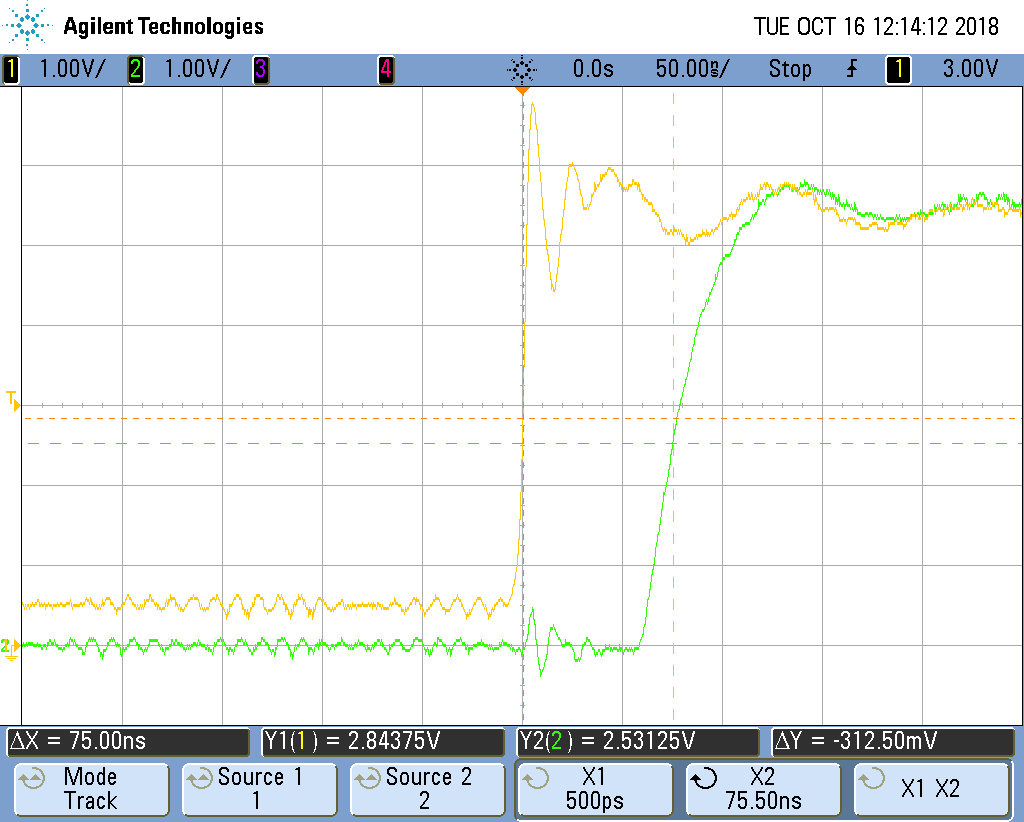
\includegraphics[width=0.6\textwidth]{figs/Ej6/sr_tplhx10.png} % first figure itself
         \caption{Medición correspondiente al tiempo de propagaci\'on de la compuerta.}
         \label{ej6_latch_imagen2}
\end{figure}
%
\noindent
De forma análoga se midieron los tiempos de fall y de propagación al pasar de 1 a cero en la salida es decir con set en 0 y reset en 1.\\
%
\noindent
Así, los tiempos que se obtuvieron se muestran en la tabla \ref{ej6_tabla_mediciones_latch} junto con los tiempos de una compuerta representativa de un latch SR comercial, de esta forma, para la comparación se utilizó la compuerta M74HC279C1R de la marca ST. 
%
\begin{table}[H]
\caption{Tabla con los valores de las mediciones tomadas (valores en nano segundos)}
\label{ej6_tabla_mediciones_latch}
\centering
\begin{tabular}{|l||l|l|l|l|}
\hline 
            & $T_{PLH}$ & $T_{PHL}$ & $T_{rise}$ & $T_{fall}$ \\ \hline \hline
Circuito    & 75        & 70        & 36.5       & 30         \\ \hline
M74HC279C1R & 20        & 20        & 15         & 15         \\ \hline
\end{tabular}
\end{table}
%
\noindent
En la tabla $T_{PLH}$ y $T_{PHL}$ refieren a los tiempos de propagación al cambiar S a uno o R a uno respectivamente.\\
Podemos ver que los valores obtenidos presentan diferencias con los valores encontrados comúnmente en la práctica, esto tiene sentido debido a que sabíamos que las compuertas utilizadas para la medición eran lentas comparadas con otras compuertas disponibles. De todas formas vemos que las mediciones se encuentran en el orden de magnitud de los valores de los componentes encontrados comercialmente.
%
\subsection{Flip Flop D}
%
\subsubsection{Funcionamiento}
\noindent
Un flip flop D se encarga de almacenar un bit, al igual que en el caso anterior, sólo que tiene una única entrada (D) y un controlador que le indica en que momento tomar el dato de dicha entrada, es decir el sistema se conecta a un clock (Clk) que le indica cuándo almacenar el valor de la entrada D.
%
\subsubsection{Circuito implementado}
\noindent
Por la naturaleza del sistema, el mismo presenta un latch SR en su interior, esto se puede ver en el esquemático del correspondiente circuito en la figura \ref{ej6_flip_flop_D}. Además posee un Edge Detector, que se encarga de detectar los flancos positivos o negativos, según sea la naturaleza del flip flop, el esquemático del mismo se encuentra en la figura \ref{ej6_flip_flop_D_edge}, el mismo corresponde a un detector de flancos negativos, se decidió por esta alternativa debido a la simpleza de implementación utilizando para realizarla un único integrado.
%
%
\begin{figure}[H]
    \centering
        \centering
        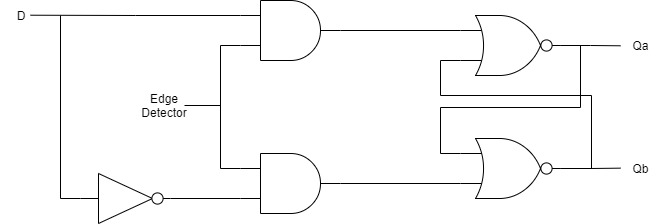
\includegraphics[width=0.8\textwidth]{figs/Ej6/flipflop.jpg} % first figure itself
         \caption{Circuito característico del Flip flop}
         \label{ej6_flip_flop_D}
\end{figure}
%
\begin{figure}[H]
    \centering
        \centering
        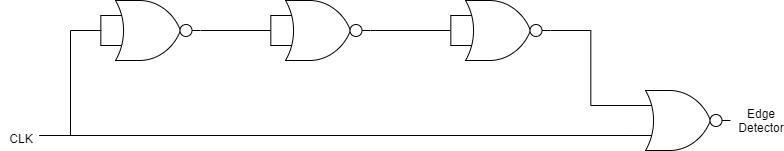
\includegraphics[width=0.8\textwidth]{figs/Ej6/Edgedetetor.jpg} % first figure itself
         \caption{Circuito implementado para la detección de flancos con pendiente negativa.}
         \label{ej6_flip_flop_D_edge}
\end{figure}
%
\noindent
De esta manera la tabla de verdad de dicho circuito se puede ver en la tabla \ref{ej6_tabla_flip_flop_D}
%
%
\begin{table}[H]
\caption{Tabla de verdad correspondiente al Flip Flop D}
\label{ej6_tabla_flip_flop_D}
\centering
\begin{tabular}{|l|l||l|l|}
\hline
D & CLK                     & Qa         & Qb         \\ \hline
0 & $\downarrow$ & 0          & 1          \\ \hline
1 & $\downarrow$ & 1          & 0          \\ \hline
X & X                       & $Qa_{-1}$ & $Qb_{-1}$ \\ \hline
\end{tabular}
\end{table}
%
\noindent
De esta manera para implementar al circuito en placa PCB se decidió utilizar los integrados 74HC08 para las compuertas And, 74HC00 para las compuertas Nand y 74HC02 para las compuertas Nor, utilizando una compuerta nor para la compuerta not que requiere el flip flop, como se puede ver en la figura \ref{ej6_flip_flop_D}.
%
\subsubsection{Mediciones y Conclusiones}
\noindent
De esta manera se procedió análogamente al caso del latch SR, es decir, se midieron los tiempos de subida y bajada a la salida de la compuerta, considerando (al igual que en el caso anterior) que el tiempo de rise o subida comienza cuando la salida vale 10\% del valor tomado como High y termina cuando vale 90\% del valor tomado como High. El caso del tiempo de bajada es análogo pero a la inversa, es decir comienza cuando la salida es 90\% del valor High y finaliza cuando el mismo es del 10\% del valor de High.\\
%
También es análogo el tratamiento de los tiempos de propagación del circuito, sólo que aquí la entrada que cambia es D es decir cuando D cambia de cero a uno se obtiene el tiempo de propagación $T_{PLH}$ y cuando la entrada D cambia de uno a cero se obtiene $T_{PHL}$, ambos tiempos medidos como en la figura \ref{ej6_latch_imagen2}, es decir desde que la señal de input alcanza el 50\% de su valor considerado como high hasta que la señal de salida del sistema llega al 50\% de su valor considerado como high.\\
%
Para los valores correspondientes a un flip flop D comercial, se decidió contrastar las mediciones tomadas con el flip flop D 74HC74, se optó por el mismo ya que se encuentra en el pañol de la facultad y es el equivalente al utilizado en el ejercicio 7 (74LS74) pero que trabaja con la misma tecnología que las compuertas utilizadas en nuestro caso, a saber, tecnología CMOS. Si bien cabe destacar que el SN74HC74 es de flanco positivo mientras que nuestro flip flop D es de flanco negativo.\\
De esta manera los resultados obtenidos de las mediciones del circuito y los que se pueden encontrar en la hoja de datos del SN74HC74 se muestran en la tabla \ref{ej6_tabla_flip_flop_mediciones}.
%
\begin{table}[H]
\caption{Valores medidos para el circuito junto a los encontrados para el Flip Flop D SN74HC74.}
\label{ej6_tabla_flip_flop_D}
\centering
\begin{tabular}{|l||l|l|l|l|}
\hline
    & $T_{PLH}$ & $T_{PHL}$ & $T_{rise}$ & $T_{fall}$ \\ \hline \hline
Circuito & 20        & 20        & 6          & 6          \\ \hline
SN74HC74 & 29        & 31        & 44         & 41         \\ \hline
\end{tabular}
\end{table}
%
\noindent
Se puede apreciar que existe una notoria diferencia entre el tiempo de rise y fall del circuito medido respecto de lo que se esperaría obtener en el integrado comercial, esto puede deberse a múltiples factores que pueden estar mejor resueltos en el integrado, debido a la cercanía de sus componentes y la facilidad del fabricante de controlar los parámetros de cada etapa a su necesidad. Además las puntas del osciloscopio hacen que la medición de dichos tiempos tan cortos se vean drásticamente modificadas, esto ya se vió en la sección destinada al Latch SR, en donde el tiempo de propagación medido con puntas x10 fue de 75ns pero medido con puntas x1 fue de 147ns.   
Con respecto a los tiempos de propagaci\'on la diferencia se encuentra dentro de lo esperado debido a las ventajas ya mencionadas que presenta el fabricante a la hora de diseñar el integrado.